\documentclass[11pt]{extarticle}
\usepackage[tmargin=1in,bmargin=1in,lmargin=1in,rmargin=1in]{geometry}
\usepackage[utf8]{inputenc}
\usepackage{tikz}
\usepackage{graphicx}
\usepackage{float}
\usepackage{setspace}
\usepackage{tabularx}
\usepackage{caption}
\usepackage{subcaption}
\usepackage{framed}
\usepackage{enumitem}
\usepackage{amsmath}
\usepackage{mathpazo}
\usepackage{ragged2e}
\usepackage{titlesec}
\usepackage{color}   %May be necessary if you want to color links
\usepackage[colorlinks = true, linkcolor=black, urlcolor=blue]{hyperref}
\usepackage{footnotebackref}
\usepackage{xcolor}
\usepackage{fancyhdr}
\usepackage{lastpage}
\usepackage{lscape}

\fancypagestyle{myheadings}
{
    \fancyhf{}
    \renewcommand{\footrulewidth}{0pt}
    \renewcommand{\headrulewidth}{0pt}
    \cfoot{Page \thepage\ of \pageref*{LastPage}}    
}

\fancypagestyle{plain}
{
    \fancyhf{}
    \chead{\small Delivery 06}
    \lhead{\small CS 353}
    \rhead{\small Spring 2022}
    % \renewcommand{\footrulewidth}{0.5pt}
    \renewcommand{\headrulewidth}{0.5pt}
    \cfoot{Page \thepage\ of \pageref*{LastPage}}    
}

\title{\textbf{Project Delivery 06}}
\author{Aliza Rafique (05986); Asad Tariq (05439); Fahad Shaikh (05452); Faiz Haseeb (06224)}
\date{$21^{st}$ March 2022}


% Set formats for each heading level
\titleformat*{\section}{\Large\bfseries\fontfamily{phv}\selectfont}
\titleformat*{\subsection}{\large\bfseries\fontfamily{phv}\selectfont}
\titleformat*{\subsubsection}{\itshape\fontfamily{phv}\selectfont}

\providecommand\phantomsection{}

\doublespacing
\begin{document}
\begin{titlepage}
\thispagestyle{empty}
\begin{center}

\includegraphics[scale=0.40]{Figures/HU-LOGO--01.jpg}
\line(1,0){400}\\
[2mm]
\fontfamily{phv}\selectfont
\textbf{Project Proposal}\\
\line(2,0){250}\\
[0.5cm]
Submitted By\\
Aliza Rafique (05986)\\
Asad Tariq (05439)\\
Fahad Shaikh (05452)\\
%Nom 2 (NI 2) \\ %À enlever le commentaire si jamais vous êtes plusieurs
[1.5cm]
CS353\\
Software Engineering\\ 
[1.0cm]
Section\\
L1\\
[1.0cm]
Instructor\\
Mohsin Nagaria\\
[1.5cm]
From the department of Computer Science\\
Dhanani School of Science and Engineering\\
Habib University\\
3$^{rd}$ February, 2022
\end{center} 
\end{titlepage}
\newpage
\thispagestyle{empty}
\tableofcontents
\hypersetup{linkcolor=blue}
\newpage
\pagestyle{plain}

\section{Layered Architecture}

\subsection{Introduction}
\begin{itemize}
    \item The layered architecture style is one of the most common architectural styles. The idea behind
    Layered Architecture is that modules or components with similar functionalities are
    organized into horizontal layers. As a result, each layer performs a specific role within the
    application.
    \item The layered architecture style does not have a restriction on the number of layers that the
    application can have, as the purpose is to have layers that promote the concept of separation of
    concerns. The layered architecture style abstracts the view of the system as a whole while
    providing enough detail to understand the roles and responsibilities of individual layers and
    the relationship between them.
\end{itemize}
\textbf{Figure} \ref{archiView}, presents an organization of the architecture in question.

\begin{figure}[H]
    \centering
    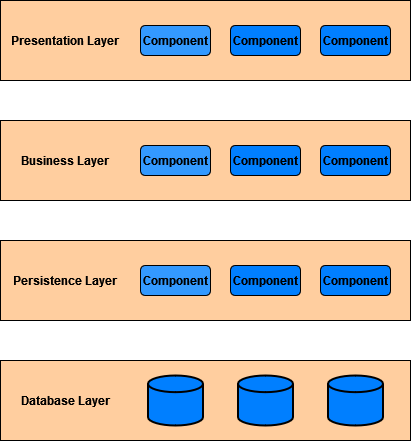
\includegraphics[width=3.5in]{Figures/layered_view_top.png}
    \caption{An organizational view of the layered architecture.}
    \label{archiView}
\end{figure}

\subsection{Topological Constraints \& Negative Behaviours}
\begin{itemize}
    \item The architecture itself is a topological constraint as it is a specific way of organizing the
    software systems.
    \item Connecters only interact with two layers, and usually, no skipping of layers is allowed.
    \item Communication is usually between one user and one interface/system.
    \item Data flow goes two ways (user to system, and back).
    \item Security can become an issue if bypassing layers is allowed. The Business Layer usually acts as
    an integrity check for passing data.
    \item If not properly designed and managed, communication between layers can become
    complicated. 
\end{itemize}

\subsection{Suitability for Application}
With respect to the our application, \textbf{Meri-Raye}, we believe the layered architecture to be the best fit for the following reasons/aspects

\subsubsection{Applicable Problems}
\begin{itemize}
    \item Software that requires separate layers of processing and security.
    \item Data driven software, CRUD applications.
\end{itemize}
Thus, with \textbf{Meri-Raye} being a review-based system, i.e., allowing controlled access to a large base of information, the layered architecture is deemed the most appropriate. 

\subsubsection{Resilience to Change}
\begin{itemize}
    \item Since the separation of concerns is the main property of the architecture, each layer of
    software has a specific function. This makes updating individual layers easy, and also allows
    teams to separate workloads.
\end{itemize}
This layered approach supports the incremental development of systems thereby, befitting the chosen development methodology that the \textbf{Meri-Raye} project is undertaking.
As a layer is developed, some of the services provided by that layer may be made available
to users.

\subsubsection{Supported Non-Functional Properties}
\begin{itemize}
    \item \textbf{Easy to implement/test}: Layered architecture is one of the easiest structures to implement.
    Since every layer has a specific function, testing is easy since layers can be mocked
    \item \textbf{Flexibility}: In some sense, any software can be abstracted into layers. Layered architecture is
    very open and broad in its implementation, thus leading to many practical applications.
    \item \textbf{Security}: Security can be implemented at every layer. If layers are skipped, extra precautions
    must be made.
\end{itemize}

\end{document}
